\documentclass[11pt,letterpaper]{article}
\usepackage{lmodern}
\usepackage[left=1.05in,right=1.05in,top=0.88in,bottom=0.92in]{geometry}
\usepackage[utf8]{inputenc}
\usepackage{amsmath,amssymb,amsthm,mathtools,booktabs,array,tabularx,microtype,xcolor}
\usepackage{tikz}
\usetikzlibrary{arrows.meta,positioning}
\usepackage[numbers,sort&compress]{natbib}
\usepackage{xurl}
\usepackage[colorlinks=true,linkcolor=blue!65!black,citecolor=blue!65!black,urlcolor=blue!65!black]{hyperref}
\hypersetup{
  pdftitle={Adaptive-Weight Sequential Calibration Beyond T^{2/3}: Deletion-Augmented Local-Trace Induction and Exact Rational Certification},
  pdfauthor={Rudra Tiwari},
  pdfsubject={Adaptive continuation weights in sign-preservation-with-reuse and sequential binary calibration}
}
\setlength{\parindent}{1.5em}
\setlength{\parskip}{0pt}
\setlength{\emergencystretch}{2em}
\setcounter{tocdepth}{2}
\newtheorem{theorem}{Theorem}[section]
\newtheorem{lemma}[theorem]{Lemma}
\newtheorem{proposition}[theorem]{Proposition}
\newtheorem{corollary}[theorem]{Corollary}
\theoremstyle{definition}
\newtheorem{definition}[theorem]{Definition}
\theoremstyle{remark}
\newtheorem{remark}[theorem]{Remark}
\newcommand{\E}{\mathbb{E}}
\newcommand{\calerr}{\operatorname{calerr}}
\newcommand{\cE}{\mathcal{E}}

\begin{document}
\thispagestyle{empty}
\begin{center}
\vspace*{0.22in}
{\LARGE\bfseries Adaptive-Weight Sequential Calibration Beyond $T^{2/3}$:\\[.15em] Deletion-Augmented Local-Trace Induction and\\[.15em] Exact Rational Certification\par}
\vspace{0.20in}
{\large State-Dependent Continuation Weights for Sign-Preservation-with-Reuse,\\[.1em] External Erasures, and Interval-Certified Exponents\par}
\vspace{0.24in}
{\normalsize\bfseries Rudra Tiwari\par}
\vspace{0.03in}
{\normalsize\itshape University of Delhi, New Delhi, India\\Inter-University Accelerator Centre (IUAC), New Delhi, India\par}
\vspace{0.10in}
{\small\href{https://orcid.org/0009-0004-8521-7627}{ORCID: 0009-0004-8521-7627}\quad|\quad\href{https://rtx09x.github.io/}{Website}\quad|\quad\href{https://github.com/Rtx09x}{GitHub}\quad|\quad\href{https://github.com/Rtx09x/Open-Research/tree/main/computer-science/sequential-calibration}{Open-Research}\par}
\vspace{0.15in}
{\normalsize November 2026\par}
\end{center}
\vspace{0.16in}
\begin{abstract}
We study classical marginal sequential calibration for binary outcomes under simultaneous-round adversarial play, using expected unnormalized $\ell_1$-calibration error $\E[\sum_{p \in P} |\sum_{t: p_t=p}(y_t - p)|]$. Building on the sign-preservation-with-reuse (SPR) framework of Qiao--Valiant and Dagan et al.\ and the $O(\log T)$-instance SPR-to-calibration transfer of Dai and Fishelson (\href{https://arxiv.org/abs/2610.07623v2}{arXiv:2610.07623v2}), we analyze an adaptive-weight recursive labeling strategy that replaces fixed continuation shifts with a causal state-dependent factor $q(z,r) = \max(1/2, U/(P_0 S - B))$ computed from observed trigger count ratios. Using exact terminating-rational parameters $\alpha = 0.0102$ and $\beta = 0.9475$ ($\varepsilon = 1-\alpha-\beta = 0.0423$), the strategy yields a candidate asymptotic calibration bound of $O(T^{20423/30846}) = O(T^{0.6620955715489852\dots})$, compared against the printed $O(T^{0.662942288})$ comparator of Dai and Fishelson. An exact 19-round transcript on $n=32$ cells shows that external erasure can let a locally full child receive another request. We account for such requests with a deletion-augmented owned-cohort trace domain $\cE(I,w)$ with recursive projection and persistent ownership. All 4,988 closed trigger-domain cells, 14,964 exact policy lookups, the 19-round witness, and the augmented projections are checked using exact arithmetic. The result is strictly asymptotic (with threshold $F=10^{10}$) and uses the published SPR transfer.
\end{abstract}
\vspace{0.10in}
\noindent\textbf{Keywords:} sequential calibration, sign-preservation-with-reuse, online forecasting, adaptive continuation weights, interval arithmetic certification, induction interface erratum.
\clearpage
\tableofcontents
\clearpage

\section{Introduction and Problem Formulation}
In sequential binary calibration~\cite{FosterVohra1998}, a forecaster chooses a finite grid $P \subset [0,1]$ and, over rounds $t=1,\dots,T$, outputs a randomized forecast $p_t \in P$ simultaneously with an adversary's outcome $y_t \in \{0,1\}$ (the adversary does not observe the realized $p_t$ before choosing $y_t$). The cumulative unnormalized $\ell_1$-calibration error is
\begin{equation}\label{eq:calerr}
  \calerr(T) = \sum_{p \in P} \left| \sum_{t: p_t = p} (y_t - p) \right|.
\end{equation}
The classical $O(T^{2/3})$ bound of Foster and Vohra~\cite{FosterVohra1998} stood for over two decades until Qiao and Valiant~\cite{QiaoValiant2021} introduced the sign-preservation game and Dagan et al.~\cite{Dagan2024} broke $T^{2/3}$ by an unspecified constant via the \emph{sign-preservation-with-reuse} (SPR) game. Recently, Dai and Fishelson~\cite{DaiFishelson2026} tightened the reduction from SPR to sequential calibration using only $O(\log T)$ SPR instances: any SPR strategy with space--time cost $O(n^\alpha t^\beta)$ where $\varepsilon = 1 - \alpha - \beta > 0$ transfers to expected calibration error
\begin{equation}\label{eq:transfer}
  \E[\calerr(T)] = O\!\left(T^{\frac{2+\varepsilon}{3+2\varepsilon}}\right) = O\!\left(T^{\frac{2}{3} - \frac{\varepsilon}{9+6\varepsilon}}\right),
\end{equation}
establishing the first explicit exponent below $2/3$, namely $O(T^{0.662942288})$ (note also concurrent work on high-dimensional calibration from harmonic weights~\cite{FishelsonMohri2026}, which addresses multi-class/multi-event dimension dependence rather than the 1D binary exponent).

\paragraph{Contribution and honest scope.}
Rather than merely retuning the fixed-shift continuation parameters of~\cite{DaiFishelson2026}, we introduce a \emph{state-dependent continuation weight} $q(z,r)$ selected causally at each epoch trigger from the observed count ratios $(z,r)$. With exact rational parameters $\alpha = 0.0102$, $\beta = 0.9475$ ($\varepsilon = 0.0423$), \eqref{eq:transfer} produces the candidate exponent
\[
  \frac{2 + 0.0423}{3 + 2(0.0423)} = \frac{2.0423}{3.0846} = \frac{20423}{30846} \approx 0.6620955715489852\dots
\]
The asymptotic bound uses the threshold $F=10^{10}$ and the SPR-to-calibration transfer~\cite{DaiFishelson2026}. Section~\ref{sec:erratum} gives an example showing why the child trace must include external erasures.

\section{The Adaptive-Weight SPR Algorithm and Rational Parameters}
In the SPR game on $n$ cells, at each round the pointer selects an empty cell $j \in [n]$ (or terminates), the labeler removes any subset of minus signs to the left of $j$ and plus signs to the right of $j$ (our strategy eagerly deletes \emph{all} eligible signs), and places $+$ or $-$ in cell $j$.

\paragraph{Algorithm $A(I,w)$.}
An instance $A(I,w)$ on a power-of-two interval $I$ carries real weight $w>0$, total request counter $\mathrm{count}$, and a current epoch $B(I,w,\tau)$ initialized with $\tau = \mathrm{count}$ at epoch start. For $|I|=1$, $A$ returns $+$ if $w \ge 1$ and $-$ otherwise. For $|I| \ge 2$, an epoch initializes two half-interval children with the same weight $w$ and counters $t_0=t_1=0$. Each incoming request increments the corresponding child's counter and is answered by that child. Letting $h=\max(t_0,t_1)$ and $\ell=\min(t_0,t_1)$, at the \emph{first} request satisfying
\begin{equation}\label{eq:trigger}
  \delta \ell \ge \tau \qquad \text{and} \qquad \ell \ge \rho h,
\end{equation}
the epoch enters a continuation phase of length $L = \lfloor \kappa h \rfloor$ (the triggering request itself is answered by the old child). Define the nominal trigger ratios
\begin{equation}\label{eq:ratios}
  z = \frac{\tau}{h}, \qquad r = \max\!\left(\rho, \frac{z}{\delta}\right),
\end{equation}
so that $(z,r)$ lies on the compact two-segment trigger domain
\begin{equation}\label{eq:domain}
  \mathcal{T} = \{(z,\rho) : 0 \le z \le \delta\rho\} \;\cup\; \{(\delta r, r) : \rho \le r \le 1\}.
\end{equation}
The next $L$ requests are answered by a new same-interval continuation instance with weight $w\cdot q(z,r)$ for a right-half trigger and $w / q(z,r)$ for a left-half trigger. Once $L$ continuation requests complete, the next request initializes a new epoch. Weights are never reset globally and physical signs are never cleared artificially upon epoch restart.

\begin{table}[!htbp]
\centering
\caption{Exact terminating-rational parameters of the adaptive-weight strategy and continuous obligations $(E)$ and $(S)$.}
\label{tab:cal-params}
\small
\begin{tabularx}{\linewidth}{@{}l l X@{}}
\toprule
\textbf{Parameter} & \textbf{Exact Rational Value} & \textbf{Role in Induction \& Certification} \\
\midrule
$\alpha, \beta$ & $0.0102,\; 0.9475$ & Space/time exponents ($\varepsilon = 1-\alpha-\beta = 0.0423$; transfer $20423/30846$) \\
$\rho, \kappa, \delta$ & $0.0097,\; 0.6,\; 14.8$ & Trigger threshold ratios and continuation length $L = \lfloor \kappa h\rfloor$ \\
$K_p, K_t$ & $0.856,\; 0.902$ & Inherited persistent and total epoch-start prefactors \\
$P_0, Q_0, q_{\max}$ & $0.85599,\; 0.9019,\; 0.76$ & Strict pre-rounding envelopes and upper cap on $q(z,r) \in [1/2, q_{\max}]$ \\
$F, C$ & $10^{10},\; F^2/K_p$ & Small-epoch cutoff ($t \le F$) and uniform induction constant \\
\bottomrule
\end{tabularx}
\end{table}

Set $H = 2^\alpha$ and $U = H \kappa^\beta$. On $\mathcal{T}$, define $S = (z+1+r+\kappa)^\beta$, $B = K_p z^\beta + r^\beta$, $P = K_p z^\beta + 1$, $A = P + r^\beta$, and
\begin{equation}\label{eq:q-def}
  q(z,r) = \max\!\left(\frac{1}{2},\; \frac{U}{P_0 S - B}\right).
\end{equation}

\begin{lemma}[Pointwise Bias-Elimination Lemma]\label{lem:bias}
Among all factors $q \in [1/2, q_{\max}]$ satisfying the completed-minus budget $B + U/q \le P_0 S$, the choice \eqref{eq:q-def} is the smallest possible. Because the plus envelopes $P + qU$ and $A + qU$ are strictly increasing in $q$, verifying the uniform domain obligations
\begin{equation}\label{eq:oblig-E}
  P_0 S - B > 0, \qquad q(z,r) \le q_{\max}, \qquad P + qU \le P_0 S, \qquad A + qU \le Q_0 S \qquad \forall (z,r) \in \mathcal{T}
\end{equation}
is both necessary and sufficient for simultaneous endpoint feasibility in $[1/2, q_{\max}]$.
\end{lemma}

With $s = 1/(1-\beta)$, $x = \min(1/\delta, K_p^{-s})$, $M = \max\bigl((((K_p+x^\beta)/(1+x)^\beta)^s+1)^{1/s}, (K_p^s + ((1+\rho^\beta)/(1+\rho)^\beta)^s)^{1/s}\bigr)$, and $D = \max\bigl((K_t^s+1)^{1/s}, (M^s + (q_{\max}H)^s)^{1/s}\bigr)$, the scalar obligations $(S)$ require
\begin{equation}\label{eq:oblig-S}
\begin{gathered}
  0 < P_0 < K_p < 1, \qquad P_0 < Q_0 < K_t, \qquad K_p \le M \le D,\\
  P_0(1+F^{-1}) + F^{-\beta} < K_p,\qquad
  Q_0(1+F^{-1}) + F^{-\beta} < K_t,\\
  D + F^{-\beta} < H.
\end{gathered}
\end{equation}

\section{External Erasures and the 19-Round Witness}\label{sec:erratum}
A recursive child may receive a sequence of requests that would be illegal in an isolated SPR game. The following transcript exhibits this phenomenon.

\begin{proposition}[Exact 19-Round Interface Witness]\label{prop:19round}
For $n=32$ and root weight $w=1$, consider the globally legal 19-round request sequence
\[
  17, 1, 18, 2, 19, 3, 20, 4, 21, 5, 22, 6, 23, 7, 24, 8, 25, 9, 25.
\]
Under the frozen exact-rational algorithm, all 19 requests are physically legal and the root never reaches full-board termination. During rounds 1--16, eight pairs trigger epochs with $\tau = 0,2,\dots,14$ and $L=\lfloor 0.6\rfloor=0$, leaving $+$ signs at cells $1,\dots,8$. At round 17 ($\tau=16$), the right child places $+$ at cell 25. At round 18, request 9 erases that $+$, yet $\delta \ell = 14.8 < 16$, so the root remains in phase one of the same epoch. Round 19 legally requests cell 25 a second time, sending the sequence $(25,25)$ to the \emph{same} right-half child and the \emph{same} previously full leaf at 25. In an isolated standalone SPR game, $(25,25)$ is illegal because the intervening erasure at round 18 is external to that child.
\end{proposition}

The exact replay in the supplement confirms that rounds 17 and 19 reach the same previously full leaf, and that the second request would be illegal in the isolated child game.  The sign bound is addressed by the enlarged domain below; see Figure~\ref{fig:trace-erasure}.

\begin{figure}[!htbp]
\centering
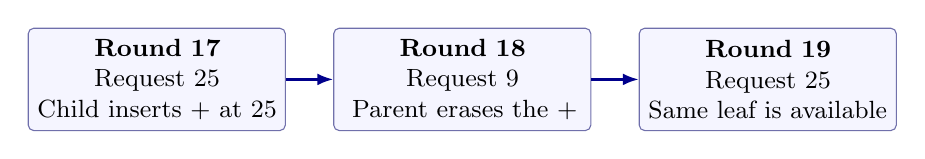
\begin{tikzpicture}[node distance=6mm, event/.style={draw=blue!40!black,draw opacity=.55,
  text opacity=1,fill=blue!4,rounded corners=2pt,align=center,text width=.25\linewidth,
  minimum height=13mm,font=\small}, link/.style={-{Latex[length=2mm]},thick,blue!55!black}]
\node[event] (a) {\textbf{Round 17}\\Request 25\\Child inserts $+$ at 25};
\node[event,right=of a] (b) {\textbf{Round 18}\\Request 9\\Parent erases the $+$};
\node[event,right=of b] (c) {\textbf{Round 19}\\Request 25\\Same leaf is available};
\draw[link] (a) -- (b);
\draw[link] (b) -- (c);
\end{tikzpicture}
\caption{The right child's projected trace includes the erasure of its owned sign at cell 25, although it receives no request at round 18. Its recursive state persists through the erasure.}
\label{fig:trace-erasure}
\end{figure}

\section{Deletion-Augmented Local-Trace Induction}
Define the enlarged trace domain on owned cohorts:

\begin{definition}[Deletion-augmented owned-cohort trace domain $\cE(I,w)$]\label{def:E-domain}
A sign is $J$-\emph{owned} if it was placed by instance $J$ or a descendant of $J$; preexisting physical signs are foreign and not counted. The domain $\cE(I,w)$ consists of all finite traces on $I$ interleaving (a)~arbitrary external erasures of owned signs (no owned insertions) and (b)~local requests at cells empty of $J$-owned signs, which eagerly erase eligible owned signs, execute the persistent subroutine $A(I,w)$, and insert the returned sign. Internal counters and recursive states persist across external erasures; a locally full owned board simply accepts no local request until an external erasure frees a cell. Only the root game enforces mandatory full-board termination.
\end{definition}

\begin{lemma}[Recursive Projection Closure]\label{lem:projection}
Every globally legal SPR transcript projects into $\cE(I,w)$ for the root, and every trace in $\cE(I,w)$ projects recursively into $\cE(I_{\mathrm{child}}, w_{\mathrm{child}})$ for every half-interval child and same-interval continuation child, preserving disjointness of earlier-epoch, phase-one, and continuation cohorts within each parent.
\end{lemma}

\begin{proof}[Projection argument]
Give each inserted sign a persistent label identifying its descendant instance and the epoch during which it was inserted. To project a trace to a child, keep the requests that the parent delegates to that child and any erasure of a sign owned by the child. A request to a sibling or to another epoch can erase a child's sign, but can add only a foreign sign. On a delegated request, the parent and child apply the same eager deletion rule to the child's owned signs: the deletion predicate uses the request position and the sign's own position and type. Local legality follows because the parent request cell contains no parent-owned sign, which includes every child-owned sign. A deletion consumes no request and does not alter the child's epoch or count. Labels are retained as a phase or epoch ends, so the surviving inherited, phase-one and continuation cohorts remain disjoint. The projection is therefore closed under the two operations in Definition~\ref{def:E-domain} and can be repeated down the recursion.
\end{proof}

\begin{theorem}[Conditional Uniform Induction Bound]\label{thm:main-cal}
Conditional on the continuous obligations \eqref{eq:oblig-E} and scalar obligations \eqref{eq:oblig-S}, for every power-of-two board size $n \ge 1$, every real weight $w>0$, every deletion-augmented trace in $\cE(I,w)$, and every request count $t \ge 0$ answered by $A(I,w)$,
\begin{equation}\label{eq:ind-bound}
  \mathrm{remaining}_+(A) \le C\, w\, n^\alpha t^\beta, \qquad
  \mathrm{remaining}_-(A) \le \frac{C}{w}\, n^\alpha t^\beta,
\end{equation}
and at the start of every epoch with prior count $\tau$, $\mathrm{persistent}_\sigma \le C w^\sigma (n/2)^\alpha K_p \tau^\beta$ and $\mathrm{total}_\sigma \le C w^\sigma (n/2)^\alpha K_t \tau^\beta$ ($\sigma \in \{+1,-1\}$). Invoking the SPR-to-calibration transfer \eqref{eq:transfer} of Dai and Fishelson~\cite{DaiFishelson2026} yields $\E[\calerr(T)] = O(T^{20423/30846})$.
\end{theorem}
\begin{proof}[Proof architecture]
Induct on $n$ and strongly on $t$ at fixed $n$, uniformly over $w>0$ and $\cE(I,w)$. At $n=1$, at most one owned sign occupies the cell at any prefix (even after repeated external erasures and re-requests) and its type obeys $w^\sigma \ge 1$. For $t \le F$, each weight change multiplies $w$ by a factor in $[1/2,2]$ and consumes a factor of at least $2$ in request count (since a continuation of length $c \le L \le h$ has parent count $\ge h+\ell+c \ge 2c$), giving $w^\sigma \ge 1/t$ and $C K_p w^\sigma n^\alpha t^\beta \ge F^2/t \ge t$. For $t > F$, at the first trigger \eqref{eq:trigger}, the half just requested is light (ties allowed), so a right trigger clears all left-child minus signs and leaves inherited signs only from the persistent inventory, together with the surviving current-epoch signs. Normalizing by $C w^\sigma (n/2)^\alpha$, surviving inventories throughout a continuation of length $c \le L$ satisfy
\[
  \mathrm{total}_- \le K_p\tau^\beta + \ell^\beta + \frac{H}{q}c^\beta, \quad
  \mathrm{persistent}_+ \le K_p\tau^\beta + h^\beta + Hq c^\beta, \quad
  \mathrm{total}_+ \le K_p\tau^\beta + h^\beta + \ell^\beta + Hq c^\beta,
\]
and symmetrically for a left trigger ($w \leftrightarrow 1/w$, $+\leftrightarrow -$). Rounding $\ell_0 \le \ell < \ell_0+1$ and $L \le L_0 < L+1$ adds at most $F^{-\beta}$ and $P_0/F$ slack, which \eqref{eq:oblig-E} and \eqref{eq:oblig-S} absorb uniformly across completed and unfinished epochs. Full case-by-case verification is given in the two proof documents in the accompanying supplement.
\end{proof}

\section{Exact Rational Certification, Limitations, and Disclosure}
The continuous trigger domain $\mathcal{T}$ is partitioned into 4,988 closed rational cells, each assigned a certified rational value of $q$ verified over the entire closed cell without floating-point rounding. The accompanying checkers verify the inequalities over each cell and the 14,964 exact endpoint and midpoint lookups. The trace checkers verify the 19-round witness and test recursive projections.
All verification files are archived at \href{https://github.com/Rtx09x/Open-Research/tree/main/computer-science/sequential-calibration}{the Open-Research calibration project} and in the accompanying supplement.

\paragraph{Limitations and disclosure.}
The bound is asymptotic, with $F=10^{10}$. This manuscript was developed with AI-assisted mathematical discovery, adversarial auditing, and exact-arithmetic verification workflows.

\bibliographystyle{plainnat}
\bibliography{references}
\end{document}
